% Cap�tulo 4
\chapter{Conclusions}\label{conclusionsChap}

On this chapter we summarize how this research was developed and present its outcomes. The phases of the work were extensively detailed over the chapters of this document and are briefly summarized on  this chapter.

We started our work by searching studies that are related to SLA and database transitions. A systematic mapping study \cite{fabioMartinSM}  was developed to answer questions like \textit{``What are the reasons to change from RDBMSs to NoSQL solutions?''}, \textit{`` How can we measure the overall improvements promised by this change?''}, \textit{``How can SLAs be used to guide database transitioning processes from RDBMSs to NoSQL databases in cloud-based apps?''}. 

As outcomes of the systematic mapping, it was found out that there is a lack of consensus and standards on how database transitions from relational DBs to NoSQL should be done, as no formal process or guidelines have been found on the literature.

Chapter \ref{bibreviewChap} discusses some of the concepts that are related with the solution proposed to the problems found on the systematic mapping. Concepts as \textit{Polyglot Persistence} and \textit{Service Level Agreements}, essential to the understanding of the proposed solution, are revealed on that chapter. 

On chapter \ref{theProblemChap} we discussed the outcomes of our systematic mapping and present extra findings that were discovered on further literature review from industry reports about database transitions in production environments. 

On the same chapter, on section \ref{theSolution}, we propose a set of SLA-based guidelines that can be used to assess and guide database transitions from relational databases to NoSQL databases. The guidelines follow a pragmatic approach and are validated on Chapter \ref{validationChap} by a case study. 

At a first moment, the validation phase searched popular open source tools where a transition might be needed, but the scope of this kind of transition became too large for the context of this work. To validate the guidelines, the core prototype of a social-media-monitoring application was built and presented on chapter \ref{validationChap}. This chapter reveals that despite some relational databases have incorporated a number of features from NoSQL technologies over the last years, sometimes even losing basic relational ACID properties, the use of a NoSQL database together with a relational database is recommended in some scenarios.


\section{Contribution}
\label{contributions}
The main contributions that emerged as results of this research are:

\begin{enumerate}
\item{A Systematic Mapping study about database transitions published on an international conference. \cite{fabioMartinSM}(Qualis/CC:B1)}
\item{Development of manpower able to work with database transition scenarios from relational databases to NoSQL environments. As NoSQL is a relatively recent concept, not many professionals are experienced with database transitioning scenarios to these technologies;}
\item{A set of guidelines to guide and assess database transitions from relational to NoSQL databases;}
\item{The core architecture, based on \textit{polyglot persistence} approach, of a social-media monitoring application. The proposed architecture enables rich user-experience features, such as suggested queries and query stemming in multiple languages, operations that are hard to be implemented in a relational-only scenario;}
\item{A set of Java-implemented load test scenarios that can be adapted to assess the QoS of applications.}

\end{enumerate}


\section{Future Works}
\label{futureWorks}
From the results of this research, the following future works can be proposed:
\begin{enumerate}
\item{Transition of (part of) a production-ready application with a large user base making use of the proposed guidelines;}
\item{Assess the performance of applications after database transitions have been performed. Verify if the guidelines were able to anticipate problems that may not be found if the guidelines weren't used;}
\item{Assess the usability of the proposed guidelines by software teams;}
\item{Write publications about the proposed guidelines in international conferences about databases, NoSLQ and Quality of Service;}
\item{Extend the proposed guidelines to enable other types of transitions in software. Assess the use of a SLA-oriented and user-oriented strategy to perform migrations of software components and services.}
\end{enumerate}


%  E os testes, devo apresentar isso nos guidelines? 
% E a vantagem de ter o Score, mostrando os posts mais relevantes primeiro?

% Even Gmail, an application that is widely used by hundreds of millions of users, may present errors and unresponsive requests when the workload is too big. After adding a single tag to all emails of an account with over 50.000 emails, for example, the user inbox can become unavailable for some moments, as image \ref{fig:gmailDown} suggests. 

% \begin{figure}[ht!]
% \centering
% 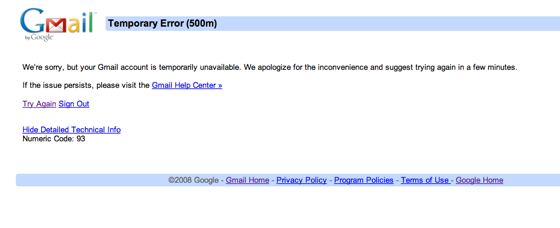
\includegraphics[width=120mm]{Imagens/gmailDown.png}
% \caption{Add a single tag on all Gmail emails.\label{fig:gmailDown}}
% \end{figure}
 
% Dizer que uma das ameacas pode ser o fator de chegada das requests nos cenarios avaliados, que podem nao representar o real. 

% TODO: Fix References: https://www.evernote.com/l/AD9tKczyJiBK9KJkJ-s1eNh-AxhMlqz3SXA

% The boundaries of this work could then be broadened to support the conception of a SLA-Guided process to support the migration/replacement of sotware components based on the cloud in future works.

% Dizer tambem que o pessoal recomenda migrar pedacos de feature a feature, como nesse case do Coursera. https://tech.coursera.org/blog/2014/09/23/courseras-adoption-of-cassandra/




% Each of these phases is composed by a number of steps, described below:
% \begin{enumerate}
% \item{Phase 1 - Identification of Case Studies \& SLAs }
%    \begin{enumerate}
%    \item {Step 1.1 - Scenario identification / Implementation: ; }
%    \item {Step 1.2 - Identification of broken SLAs: We need to identify that the a set a constraints (i.e: execution time of a query) is not being met by the current architecture;}
%    \item {Step 1.3 - Implementation of ``runnable SLAs'' : On this step we will implement executable versions of the SLA identified on the previous step. These ``runnable SLAs" will be used to verify that a set of constraints is not being met by the current architecture. }
%    \item {Step 1.4 - Execution reports: After an executable SLA has been identified and implemented, execution reports will be consolidated to prove that the constraints of the SLA are being broken by the current architecture of the scenario.}

%    \end{enumerate}


% \item{Phase 2 - Plan}
%    \begin{enumerate}
%    \item{Step 2.1 - Literature Review for each scenario: We will evaluate and search for solutions on how each scenario can make use of a NoSQL Database to meet the desired SLA; }
%    \item{Step 2.2 - Survey of industry experts: We will survey industry experts on how they would propose a NoSQL architecture to solve the problem described on each scenario. }
%    \end{enumerate}

% \item{Phase 3 - Do}
%    \begin{enumerate}
%    \item{Step 3.1 - Planning of changes: We will gather the results from the previous phase and design the changes that will be performed on each scenario;}
%    \item{Step 3.2 - Implementation: We will implement the changes identified on the previous step. }
%    \end{enumerate}

% \item{Phase 4 - Check}
%    \begin{enumerate}
%    \item {Step 4.1 - New Execution Reports: The same SLAs identified on the first step will be run on the modified scenarios, and execution reports will be consolidated.}
%    \item {Step 4.2 - Comparison of Results: The reports extracted on steps 4.1 and 1.4 will be compared to check if the changes made on Phase 3 satisfied the proposed SLA.}
%    \end{enumerate}

% \item{Phase 5 - Act}
%    \begin{enumerate}
%    \item{Step 5.1 - Tweaks on the proposed architecture: If the SLA isn't being met yet, new changes might be needed, and on this step we join together the phases 2, 3 and 4 to iterate over the needed changes. }
%    \end{enumerate}


% \item{Phase 6 - Final Results}
%    \begin{enumerate}
%    \item{Step 6.1 - Publish the results: We will submit the results of this study to academical conferences to have feedback from the community. }
%    \item{Step 6.2 - Write the final results: All the documents produced by our study and a final dissertation will be sent to the Universidade Federal do Rio Grande do Norte (UFRN).}
%    \end{enumerate}

% \section{Schedule}

% A detailed view of the execution flow of our steps can be seen on Figure~\ref{fig:schedule}. 
% \begin{figure}[ht!]
% \centering
% 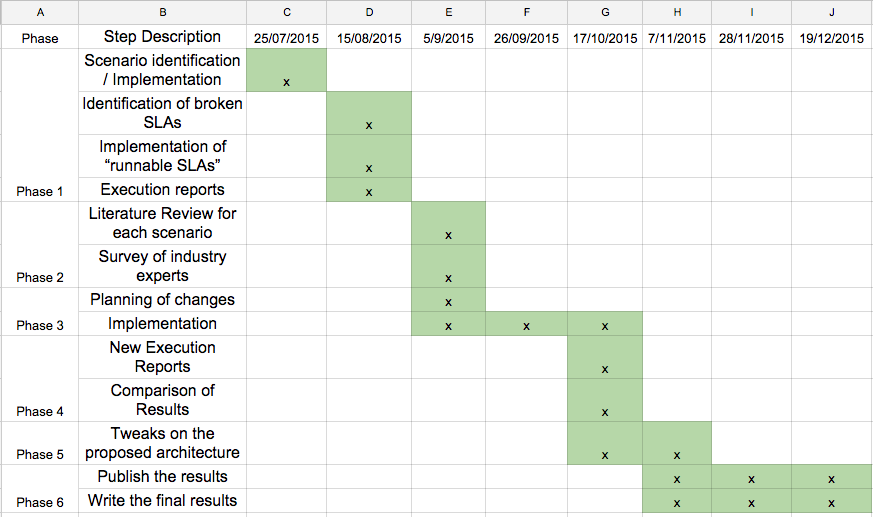
\includegraphics[width=140mm]{schedule.png}
% \caption{Schedule.\label{fig:schedule}}
% \end{figure}
% \end{enumerate}